%-*- coding:utf-8 -*-

\begin{frame}[t,fragile]{自己相関時間と統計誤差}
  \begin{itemize}
    %\setlength{\itemsep}{1em}
  \item \(M\) を固定して \(n\) を増やし、\(n\gg\tau_{\mathrm{int}}\) で
    \(\left(\sigma^{(n)}\right)^2\) がほぼ一定になる範囲を探す。
    その一定値の平方根 \(\sigma^{(\infty)}\) を平均値の標準誤差とする
  
  \item ビン幅を大きくしすぎるとビン数が減り、誤差の推定自体が不安定になる。ビン数は、最低でも10程度を残すことを目安とする
  \end{itemize}

  \hspace*{4em} 自己相関時間 \hspace*{9em} 統計誤差

  \noindent\resizebox{0.49\textwidth}{!}{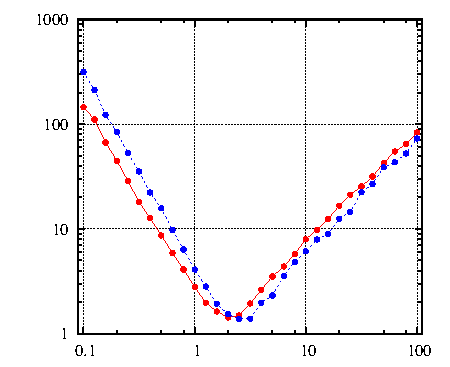
\includegraphics{image/autocorr.pdf}}
  \resizebox{0.49\textwidth}{!}{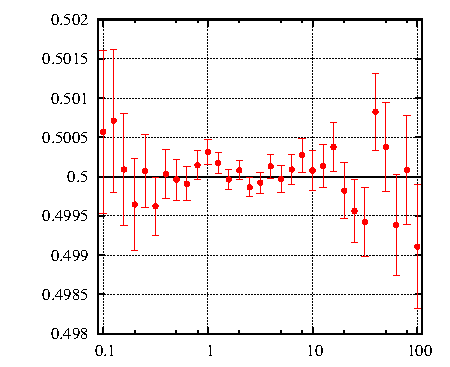
\includegraphics{image/error.pdf}}

  \hspace*{7em} $\Delta$ \hspace*{12em} $\Delta$
\end{frame}
